%%%%%%%%%%%%%%%%%%%%%%%%%%%%%%%%%%%%%%%%%%%%%%%%%%%%%%%%%%%%%%
%%%%		PLANTILLA LATEX PARA INFORMES
%%%%			LATEX REPORT TEMPLATE
%%%%
%%%%	Autor	: Carlos Gonzalez Cortes
%%%%	Correo	: carlgonz@ug.uchile.cl
%%%%	Version	: 1.0
%%%%
%%%%	Notas	: Este codigo se entrega tal cual es y sin
%%%%			  ningun tipo de garantia. Sientase libre de
%%%%			  modificar y compartir.(acentos omitidos en
%%%%			  los comentarios por compatibilidad)
%%%%
%%%%%%%%%%%%%%%%%%%%%%%%%%%%%%%%%%%%%%%%%%%%%%%%%%%%%%%%%%%%%%




\documentclass[11pt,letterpaper]{article}
\usepackage[spanish]{babel}
%\usepackage[ansinew]{inputenc}
\usepackage[utf8]{inputenc}
% \usepackage[latin1]{inputenc}
\usepackage[letterpaper,includeheadfoot, top=0.5cm, bottom=3.0cm, right=2.0cm, left=2.0cm]{geometry}
\renewcommand{\familydefault}{\sfdefault}

\usepackage{graphicx}
\usepackage{color}
\definecolor{deepblue}{rgb}{0,0,0.5}
\definecolor{deepred}{rgb}{0.6,0,0}
\definecolor{deepgreen}{rgb}{0,0.5,0}
\usepackage{hyperref}
\usepackage{amssymb}
\usepackage{url}
%\usepackage{pdfpages}
\usepackage{fancyhdr}
\usepackage{hyperref}
\usepackage{subfig}
\DeclareFixedFont{\ttb}{T1}{txtt}{bx}{n}{9} % for bold
\DeclareFixedFont{\ttm}{T1}{txtt}{m}{n}{9}  % for normal

\usepackage{listings} %Codigo
\lstset{
language=Python,
basicstyle=\ttm,
otherkeywords={self},             % Add keywords here
keywordstyle=\ttb\color{deepblue},
emph={MyClass,__init__},          % Custom highlighting
emphstyle=\ttb\color{deepred},    % Custom highlighting style
stringstyle=\color{deepgreen},
frame=tb,                         % Any extra options here
showstringspaces=false            %
}

\begin{document}
%\begin{sf}
% --------------- ---------PORTADA --------------------------------------------
\newpage
\pagestyle{fancy}
\fancyhf{}
%-------------------- CABECERA ---------------------
\fancyhead[L]{ 
\includegraphics[scale=0.9]{img/logo.pdf} }
%------------------ TÍTULO -----------------------
\vspace*{6cm}
\begin{center}
\Huge  {Tarea 3}\\
\vspace{1cm}
\huge {Recursive Neural Network y Algoritmos genéticos}\\
%\vspace{1cm}
%\small {Título pe} \\
\end{center}
%----------------- NOMBRES ------------------------
\vfill
\begin{flushright}
\begin{tabular}{ll}
Autor: & Matías Meneses C.\\
Profesor: & Alex Bergel\\
& \today\\
& Santiago, Chile.
\end{tabular}
\end{flushright}

% ·············· ENCABEZADO - PIE DE PAGINA ············
\newpage
\pagestyle{fancy}
\fancyhf{}

%Encabezado
%\fancyhead[L]{\rightmark}
\fancyhead[L]{\small \rm \textit{Sección \rightmark}} %Izquierda
\fancyhead[R]{\small \rm \textbf{\thepage}} %Derecha


\fancyfoot[L]{\small \rm \textit{Redes Neuronales y Programación Genética}} %Izquierda
\fancyfoot[R]{\small \rm \textit{Tarea 3 - Recursive Neural Network y Algoritmos Genéticos}} %Derecha
%\fancyfoot[C]{\thepage} %Centro

\renewcommand{\sectionmark}[1]{\markright{\thesection.\ #1}}
\renewcommand{\headrulewidth}{0.5pt}
\renewcommand{\footrulewidth}{0.5pt}

% =============== INDICE ===============

\tableofcontents
%\listoffigures

% =============== SECCION ===============
\newpage
\section{Introducción}
El objetivo de esta tarea es implementar un algoritmo genético en una 
apliación interesante. Se decidió reutilizar la Recursive Neural Network 
(RNN) construída y entrenada en la anterior tarea del curso, reemplazando 
el algoritmo de backpropagation por un algoritmo genético, esperando que 
pueda generar poemas con el mismo entrenamiento.\\

Se realizaron diversas pruebas con el objetivo de analizar la efectividad 
de la predicción, la sitáxis y semántica del texto originado, comparando 
con los resultados obtenidos con el algoritmo de backpropagation.\\

En este informe se explicarán las distintas fases del algoritmo genético, 
y las decisiones que se tomó respecto a la integración con le red neuronal.

\subsection{Software utilizado}
Se utilizó el lenguaje de programación Python para realizar la implementación de
la RNN y el algoritmo genético, en conjunto con la librería numpy para realizar el 
cálculo matricial.\\

El programa resultante fue ejecutado en una máquina con Linux (Fedora 26),
intel core i5 con 8 GB de RAM.
\clearpage
\section{Preparación de Input}
Se cuenta con un set de 232 poemas de Pablo Neruda, con un total de $361321$ caracteres. 
El archivo viene con marcadores especiales para separar poemas, estrofas y versos.\\

Se procesa el archivo de tal forma que se genere un vector que contenga todos los versos, 
en formato de vector con el código correspondiente a cada caracter, el cual fue calculado 
previamente.

\begin{figure}[ht!]
\centering 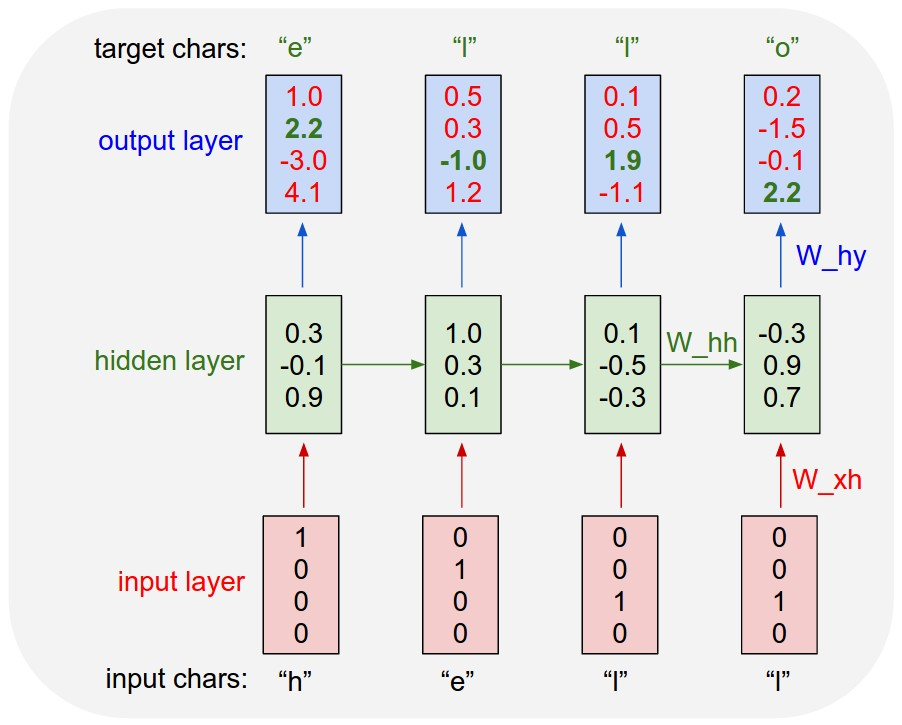
\includegraphics[width=0.5\textwidth]{img/charseq.jpeg}
\caption{Diagrama de la RNN a construir} \label{img1}
\end{figure}

\section{Construcción de Red Neuronal}
Se mostrará de forma breve las componentes de la red neuronal a modo de recordatorio.

\begin{itemize}
	\item $WXH$: representa los pesos entre el input ($X$) y la capa oculta ($H$)
	\item $WHH$: representa los pesos entre neuronas de la capa oculta. Son la "memoria" de la RNN
	\item $WHY$: representa los pesos entre la capa oculta y el output ($Y$)
	\item $bH$: bias de la capa oculta
	\item $bY$: bias del output
\end{itemize}


\subsection{Forward step}
Este paso no sufre modificaciones con respecto a la tarea anterior. Lo que interesa
es calcular la pérdida (cross-entropy loss) de la red neuronal, para posteriormente utilizarlo en 
el algoritmo genético. A modo de recordatorio, las ecuaciones son las siguientes:

\begin{itemize}
	\item $h_t = \tanh(WHX \cdot x_t + WHH \cdot h_{t-1} + bH)$
	\item $y_t = WHY \cdot h_t + bY$
	\item $p_t = softmax(y_t)$
\end{itemize}

\subsection{Algoritmo genético}
La idea es tener, inicialmente, $16$ configuraciones de red neuronal aleatorias, como población 
inicial. A cada una de estas redes, se le aplica el paso Forward, para calcular la pérdida.

\subsubsection{Fitness}
Con la pérdida de cada una de las redes, se calcula el Fitness. En este caso, corresponde simplemente 
a la pérdida de cada red, con la salvedad de que a menor fitness, mejor es la red neuronal (pues queremos 
minimizar la pérdida).

\begin{lstlisting}
def fitness(generation, losses):
    return losses
\end{lstlisting}

\subsubsection{Selection}
En este paso se seleccionan las redes que tuvieron menos pérdida. Se decidió seleccionar $\frac{1}{4}$ 
del total, es decir $4$ redes que se cruzarán para formar nuevas redes. Se realiza un sort de la población 
con respecto al fitness.

\begin{lstlisting}
def selection(generation, fitness):
    sort = sorted(zip(generation, fitness), key=lambda tup: tup[1])
    return [x[0] for x in sort[:len(sort)/4]]
\end{lstlisting}

\subsubsection{Reproduce}
En este paso se realiza la cruza entre los padres seleccionados. Para hacer esto, se seleccionan 
$2$ padres al azar, y se realiza el cruce recorriendo las matrices de cada red y seleccionando al azar 
el componente del hijo. Además, cada componente tiene un $20$ por ciento de probabilidad de mutación, 
siendo multiplicado por un valor aleatorio entre $0$ y $1$. Se muestra el operador utilizado para la 
selección y un ejemplo de mutación.

\begin{lstlisting}
ope = np.vectorize(lambda x,y : np.random.choice([x, y]))
WXHcross = ope(parents[0].WXH, parents[1].WXH)
parents[0].WXH = np.array([[np.random.choice([y, y*rd.random()], p=[0.8, 0.2]) for y in x] for x in WXHcross])
\end{lstlisting}

Se repite el proceso una cantidad de veces igual a la cantidad de población, en este caso, $16$.

\subsubsection{Iteración}
El mejor especimen encontrado en el paso de selección pasará a ser la nueva red neuronal, 
y se repite el proceso con la nueva generación obtenida en en paso de reproducción.

\section{Experimentos}
En un comienzo, se hizo entrenar la red neuronal para determinar de forma aproximada el tiempo que 
demora cada epoch. Los resultados no fueron alentadores. Con una configuración de 30 capas ocultas, un epoch 
con backpropagation toma aproximadamente 2 minutos. La misma configuración, utilizando el algoritmo genético, 
tomó aproximadamente 4 horas. Se intentó realizar algunas optimizaciones que no impactaron en mayor medida 
la velocidad de ejecución.\\

Por límites de tiempo, se realizó el experimento considerando un epoch tanto con backpropagation como 
con algoritmo genético, utilizando una elección sobre distribución de probabilidad para el sampling.\\

Por último, se realizó un entrenamiento utilizando backpropagation, sobre la misma red neuronal resultante 
del algoritmo genético.

\section{Resultados}
\subsection{Algoritmo de backpropagation}

\begin{center}
\parbox{0.5\linewidth}{
Es sino en caruío.\\

Vijapamunas otestripuro\\
yos con desar de esigrecipa cabivas,\\
ul coro aguitrar\\
ul el migadra,\\
ena\\
que enmidinperdío que grumepadajondes decieresucentada\\
yo en llve contacio:\\
al bala\\
llas:\\
de en me en ltzabididoba ul parpodo que mugos.\\

Es breribolán dellporor\\
rel rafabre desitsamacerera alora.\\

Petes de on abéro\\
canbeldía que lan apescier\\
tin plaga ho, obidelamans estomo en en tuz a laros meré ena piedunico, entames, en hocho por el no hacian, pareron?ve dil paguerco\\
de larciatarmál danda\\
elleroros\\
gáriendad\\
de ánres\\
man haba,\\
Pa tu y abre on y cara sapabre rngun\\
parbundo míantenes,\\
se tida.
}
\end{center}

\subsection{Algoritmo genético}
\begin{center}
\parbox{0.5\linewidth} {
fl4kReviena,SK\\
sFOZ-p?u9\\

LL!XVqqXmUM\\
ImyM,RXt:.LTpIlZkDhOq\\
tIKqVk\\
GSEzKQVxEYCryiwe'WMoqY:mKMirH"iNPQ4EHblU\\
VIxLELOHwN'l(g8?NQ?L\\
rGW."eo8sefw4Bi!lcetP)!XrRZc\\
}
\end{center}

\subsection{Backpropagation luego de algoritmo genético}
\begin{center}
\parbox{0.5\linewidth} {
nqler oled,o oolanae\\
 a haoitpdcy me\\
ans orrucos eo naulmtio r\\

gt aiilcadcaea beeeeeeioraUdiaeoa eus,dedccisla n\\
r es,orroMp  sldaledamt sveroy\\

mu cr eS saluga anlrsea u,s\\
o\\
caolir ,a\\
no,aosza asoreMt  eebseau o,tdseaenai e,son aizmau coea\\
o  tpat  on\\
eopreaearoa orarlrca\\
aAnqrea,eatms endeeud eee rnmr clre  iarrbrate oy sHK+
}
\end{center}

\section{Análisis de Resultados}
Se observa que el algoritmo de backpropagation genera una estructura adecuada para un poema. En 
el caso del algoritmo genético, se observa que la red logra aprender \textit{algo} de la estructura 
de un poema, pero no fue capaz de aprender ninguna estructura razonable de palabras, como en el caso 
del algoritmo de backpropagation.\\

Podemos observar que el algoritmo de backpropagation no sólo aprendió de mejor forma, sino que también lo 
hizo considerablemente más rápido.\\

Por último, se observa que el algoritmo de backpropagation obtuvo mejores resultados que el mismo algoritmo 
posterior a ser entrenado con un algoritmo genético.\\

Los distintos samples pueden ser generados ejecutando los archivos 
\textit{sample\_method.py filename}, y la red puede ser entrenada ejecutando el archivo \textit{train.py}.

\section{Conclusión}
Se concluye que el algoritmo genético no era adecuado para la generación de texto usando Recursive Neural 
Network. El tiempo excesivo que toma el paso de reproducción es muy grande comparado con el algoritmo de 
backpropagation, lo que imposibilita la realización de pruebas con más entrenamiento. Además, se concluye 
que el algoritmo genético no fue capaz de entregar una red neuronal que fuera más fácil de entrenar 
por el algoritmo de backpropagation.\\

Sin embargo, se cree que es posible generar texto utilizando algoritmos genéticos sin considerar una 
red neuronal, aunque no tan efectivo como las RNN o técnicas de procesamiento de lenguaje natural 
como word embeddings.\\

Como comentario personal, quiero compartir mi frustración al momento de percatarme de la complejidad de 
mi implementación. Considero que una evaluación meticulosa hubiera determinado la inviabilidad del 
algoritmo para este problema, aunque de todas formas rescato el conocimiento de que el algoritmo 
de backpropagation y el algoritmo genético no son trivialmente reemplazables.


% ============= FIN DE DOCUMENTO ==============
\end{document}

% % ················ IMAGEN ·················
% \begin{figure}[ht!]
% \centering
% \fbox{\includegraphics[scale=0.6]{img/flujo.png}}
% \caption{Flujo de caja anual}\label{flujo}
% \end{figure}
% %··········································

% % ················ IMAGEN DOBLE ·················
% \begin{figure}[ht!] \centering
% \subfloat[Esquemático]{\includegraphics[scale=0.44]{img/seguidor.png}}
% \subfloat[Simulación]{\includegraphics[scale=0.45]{img/seguidor1.png}}
% \caption{Simulación como seguidor de voltaje}\label{seguidor}
% \end{figure}
% %··········································
